\documentclass[tikz,border=2pt]{standalone}
\usepackage{amsmath}
\usepackage{pgfplots}
\pgfplotsset{compat=1.18}
\usetikzlibrary{arrows.meta}
\begin{document}
% Example 6.2 (max 3x1+5x2, x1<=4, 2x2<=12, 3x1+2x2<=18): at the corner (0,6), basis {3,2,5}, the objective row
% reads Z = 30 + 3x1 - (5/2)x4; reduced cost of x1 is -3 < 0, so raising x1 along the edge 2x2=12 improves Z up to (2,6), Z=36;
% reduced cost of x4 is 5/2 >= 0, raising x4 (moving down along x1=0) lowers Z. At (2,6) the line 3x1+5x2=36 touches the region.
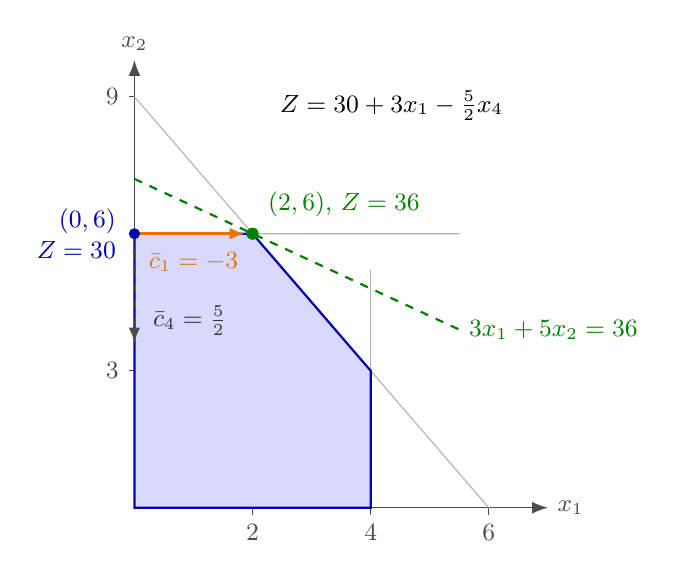
\begin{tikzpicture}[font=\small, >={Latex[length=2mm]}, x=0.75cm, y=0.58cm]
  \fill[blue!15] (0,0) -- (4,0) -- (4,3) -- (2,6) -- (0,6) -- cycle;
  \draw[->, gray!60!black] (0,0) -- (7,0) node[anchor=west] {$x_1$};
  \draw[->, gray!60!black] (0,0) -- (0,9.8) node[anchor=south] {$x_2$};
  \foreach \x in {2,4,6} \draw[gray!60!black] (\x,0) -- (\x,-0.15) node[anchor=north] {$\x$};
  \foreach \y in {3,9} \draw[gray!60!black] (0,\y) -- (-0.1,\y) node[anchor=east] {$\y$};
  \draw[gray!60, thin] (4,0) -- (4,5.2) (0,9) -- (6,0) (0,6) -- (5.5,6);
  \draw[blue!70!black, thick] (0,0) -- (4,0) -- (4,3) -- (2,6) -- (0,6) -- cycle;
  % objective line through the optimum
  \draw[green!50!black, thick, dashed] (0,7.2) -- (5.5,3.9);
  \node[green!50!black, anchor=west] at (5.5,3.9) {$3x_1+5x_2=36$};
  % the two edges at (0,6)
  \draw[->, orange!90!black, very thick] (0,6) -- (1.88,6);
  \node[orange!90!black, anchor=north] at (1.0,5.8) {$\bar{c}_1=-3$};
  \draw[->, gray!60!black, very thick, dashed] (0,6) -- (0,3.6);
  \node[gray!40!black, anchor=west] at (0.15,4.1) {$\bar{c}_4=\tfrac{5}{2}$};
  % points
  \fill[blue!70!black] (0,6) circle (2pt);
  \fill[green!50!black] (2,6) circle (2.2pt);
  \node[blue!70!black, anchor=east, align=right] at (-0.15,6) {$(0,6)$\\ $Z=30$};
  \node[green!50!black, anchor=south west] at (2.1,6.15) {$(2,6)$, $Z=36$};
  % objective row at (0,6)
  \node[anchor=west] at (2.3,8.8) {$Z=30+3x_1-\tfrac{5}{2}x_4$};
\end{tikzpicture}
\end{document}
